\documentclass[12pt,a4paper,fleqn]{article}
\title{Progress Report}
\author{Syed Ahmad Raza}
\date{2016.12.13}
\usepackage{mathtools}
\usepackage{graphicx}
\usepackage{color}          % for color eps output

\begin{document}
\maketitle \section*{Numerical differentiation using arrays for the first
derivative}
Arrays were utilized in an algorithm coded in C++ for numerical differentiation
using three different commonly used schemes. The function sin$(3x)$ was
differentiated using forward difference, backward difference and central
difference methods.

\subsection*{Forward difference method}
\begin{equation}
f^\prime(x) = \frac{f(x_{i+1})-f(x_i)}{x_{i+1}-x_i}
\end{equation}

\subsection*{Backward difference method}
\begin{equation}
f^\prime(x) = \frac{f(x_i)-f(x_{i-1})}{x_i-x_{i-1}}
\end{equation}

\subsection*{Central difference method}
\begin{equation}
f^\prime(x) = \frac{f(x_{i+1})-f(x_{i-1})}{x_{i+1}-x_{i-1}}
\end{equation}

The results are shown in the figures below.

\begin{figure}[p!]
\centering
% GNUPLOT: LaTeX picture with Postscript
\begingroup
  \makeatletter
  \providecommand\color[2][]{%
    \GenericError{(gnuplot) \space\space\space\@spaces}{%
      Package color not loaded in conjunction with
      terminal option `colourtext'%
    }{See the gnuplot documentation for explanation.%
    }{Either use 'blacktext' in gnuplot or load the package
      color.sty in LaTeX.}%
    \renewcommand\color[2][]{}%
  }%
  \providecommand\includegraphics[2][]{%
    \GenericError{(gnuplot) \space\space\space\@spaces}{%
      Package graphicx or graphics not loaded%
    }{See the gnuplot documentation for explanation.%
    }{The gnuplot epslatex terminal needs graphicx.sty or graphics.sty.}%
    \renewcommand\includegraphics[2][]{}%
  }%
  \providecommand\rotatebox[2]{#2}%
  \@ifundefined{ifGPcolor}{%
    \newif\ifGPcolor
    \GPcolortrue
  }{}%
  \@ifundefined{ifGPblacktext}{%
    \newif\ifGPblacktext
    \GPblacktextfalse
  }{}%
  % define a \g@addto@macro without @ in the name:
  \let\gplgaddtomacro\g@addto@macro
  % define empty templates for all commands taking text:
  \gdef\gplbacktext{}%
  \gdef\gplfronttext{}%
  \makeatother
  \ifGPblacktext
    % no textcolor at all
    \def\colorrgb#1{}%
    \def\colorgray#1{}%
  \else
    % gray or color?
    \ifGPcolor
      \def\colorrgb#1{\color[rgb]{#1}}%
      \def\colorgray#1{\color[gray]{#1}}%
      \expandafter\def\csname LTw\endcsname{\color{white}}%
      \expandafter\def\csname LTb\endcsname{\color{black}}%
      \expandafter\def\csname LTa\endcsname{\color{black}}%
      \expandafter\def\csname LT0\endcsname{\color[rgb]{1,0,0}}%
      \expandafter\def\csname LT1\endcsname{\color[rgb]{0,1,0}}%
      \expandafter\def\csname LT2\endcsname{\color[rgb]{0,0,1}}%
      \expandafter\def\csname LT3\endcsname{\color[rgb]{1,0,1}}%
      \expandafter\def\csname LT4\endcsname{\color[rgb]{0,1,1}}%
      \expandafter\def\csname LT5\endcsname{\color[rgb]{1,1,0}}%
      \expandafter\def\csname LT6\endcsname{\color[rgb]{0,0,0}}%
      \expandafter\def\csname LT7\endcsname{\color[rgb]{1,0.3,0}}%
      \expandafter\def\csname LT8\endcsname{\color[rgb]{0.5,0.5,0.5}}%
    \else
      % gray
      \def\colorrgb#1{\color{black}}%
      \def\colorgray#1{\color[gray]{#1}}%
      \expandafter\def\csname LTw\endcsname{\color{white}}%
      \expandafter\def\csname LTb\endcsname{\color{black}}%
      \expandafter\def\csname LTa\endcsname{\color{black}}%
      \expandafter\def\csname LT0\endcsname{\color{black}}%
      \expandafter\def\csname LT1\endcsname{\color{black}}%
      \expandafter\def\csname LT2\endcsname{\color{black}}%
      \expandafter\def\csname LT3\endcsname{\color{black}}%
      \expandafter\def\csname LT4\endcsname{\color{black}}%
      \expandafter\def\csname LT5\endcsname{\color{black}}%
      \expandafter\def\csname LT6\endcsname{\color{black}}%
      \expandafter\def\csname LT7\endcsname{\color{black}}%
      \expandafter\def\csname LT8\endcsname{\color{black}}%
    \fi
  \fi
    \setlength{\unitlength}{0.0500bp}%
    \ifx\gptboxheight\undefined%
      \newlength{\gptboxheight}%
      \newlength{\gptboxwidth}%
      \newsavebox{\gptboxtext}%
    \fi%
    \setlength{\fboxrule}{0.5pt}%
    \setlength{\fboxsep}{1pt}%
\begin{picture}(7766.00,7766.00)%
    \gplgaddtomacro\gplbacktext{%
      \csname LTb\endcsname%
      \put(682,704){\makebox(0,0)[r]{\strut{}$-3$}}%
      \put(682,1837){\makebox(0,0)[r]{\strut{}$-2$}}%
      \put(682,2970){\makebox(0,0)[r]{\strut{}$-1$}}%
      \put(682,4102){\makebox(0,0)[r]{\strut{}$0$}}%
      \put(682,5235){\makebox(0,0)[r]{\strut{}$1$}}%
      \put(682,6368){\makebox(0,0)[r]{\strut{}$2$}}%
      \put(682,7501){\makebox(0,0)[r]{\strut{}$3$}}%
      \put(814,484){\makebox(0,0){\strut{}$0$}}%
      \put(2453,484){\makebox(0,0){\strut{}$\pi/4$}}%
      \put(4091,484){\makebox(0,0){\strut{}$\pi/2$}}%
      \put(5730,484){\makebox(0,0){\strut{}$3\pi/4$}}%
      \put(7369,484){\makebox(0,0){\strut{}$\pi$}}%
    }%
    \gplgaddtomacro\gplfronttext{%
      \csname LTb\endcsname%
      \put(176,4102){\rotatebox{-270}{\makebox(0,0){\strut{}$f(x)$}}}%
      \put(4091,154){\makebox(0,0){\strut{}$x$}}%
      \csname LTb\endcsname%
      \put(5471,1727){\makebox(0,0)[r]{\strut{}Analytical}}%
      \csname LTb\endcsname%
      \put(5471,1507){\makebox(0,0)[r]{\strut{}Forward}}%
      \csname LTb\endcsname%
      \put(5471,1287){\makebox(0,0)[r]{\strut{}Backward}}%
      \csname LTb\endcsname%
      \put(5471,1067){\makebox(0,0)[r]{\strut{}Central}}%
    }%
    \gplbacktext
    \put(0,0){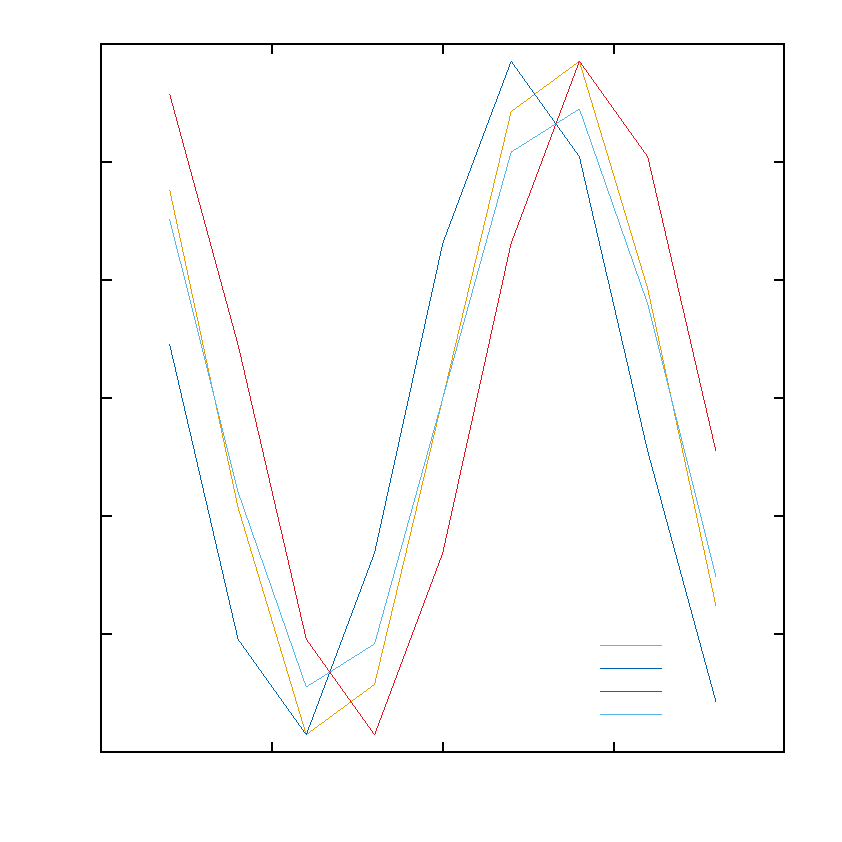
\includegraphics{D:/PhD/Tasks/004/report/firstsin10}}%
    \gplfronttext
  \end{picture}%
\endgroup

\caption{Comparison of numerical differentiation of sin$(3x)$ using 10 intervals
for the first derivative}
\end{figure}
\begin{figure}[p!]
\centering
% GNUPLOT: LaTeX picture with Postscript
\begingroup
  \makeatletter
  \providecommand\color[2][]{%
    \GenericError{(gnuplot) \space\space\space\@spaces}{%
      Package color not loaded in conjunction with
      terminal option `colourtext'%
    }{See the gnuplot documentation for explanation.%
    }{Either use 'blacktext' in gnuplot or load the package
      color.sty in LaTeX.}%
    \renewcommand\color[2][]{}%
  }%
  \providecommand\includegraphics[2][]{%
    \GenericError{(gnuplot) \space\space\space\@spaces}{%
      Package graphicx or graphics not loaded%
    }{See the gnuplot documentation for explanation.%
    }{The gnuplot epslatex terminal needs graphicx.sty or graphics.sty.}%
    \renewcommand\includegraphics[2][]{}%
  }%
  \providecommand\rotatebox[2]{#2}%
  \@ifundefined{ifGPcolor}{%
    \newif\ifGPcolor
    \GPcolortrue
  }{}%
  \@ifundefined{ifGPblacktext}{%
    \newif\ifGPblacktext
    \GPblacktextfalse
  }{}%
  % define a \g@addto@macro without @ in the name:
  \let\gplgaddtomacro\g@addto@macro
  % define empty templates for all commands taking text:
  \gdef\gplbacktext{}%
  \gdef\gplfronttext{}%
  \makeatother
  \ifGPblacktext
    % no textcolor at all
    \def\colorrgb#1{}%
    \def\colorgray#1{}%
  \else
    % gray or color?
    \ifGPcolor
      \def\colorrgb#1{\color[rgb]{#1}}%
      \def\colorgray#1{\color[gray]{#1}}%
      \expandafter\def\csname LTw\endcsname{\color{white}}%
      \expandafter\def\csname LTb\endcsname{\color{black}}%
      \expandafter\def\csname LTa\endcsname{\color{black}}%
      \expandafter\def\csname LT0\endcsname{\color[rgb]{1,0,0}}%
      \expandafter\def\csname LT1\endcsname{\color[rgb]{0,1,0}}%
      \expandafter\def\csname LT2\endcsname{\color[rgb]{0,0,1}}%
      \expandafter\def\csname LT3\endcsname{\color[rgb]{1,0,1}}%
      \expandafter\def\csname LT4\endcsname{\color[rgb]{0,1,1}}%
      \expandafter\def\csname LT5\endcsname{\color[rgb]{1,1,0}}%
      \expandafter\def\csname LT6\endcsname{\color[rgb]{0,0,0}}%
      \expandafter\def\csname LT7\endcsname{\color[rgb]{1,0.3,0}}%
      \expandafter\def\csname LT8\endcsname{\color[rgb]{0.5,0.5,0.5}}%
    \else
      % gray
      \def\colorrgb#1{\color{black}}%
      \def\colorgray#1{\color[gray]{#1}}%
      \expandafter\def\csname LTw\endcsname{\color{white}}%
      \expandafter\def\csname LTb\endcsname{\color{black}}%
      \expandafter\def\csname LTa\endcsname{\color{black}}%
      \expandafter\def\csname LT0\endcsname{\color{black}}%
      \expandafter\def\csname LT1\endcsname{\color{black}}%
      \expandafter\def\csname LT2\endcsname{\color{black}}%
      \expandafter\def\csname LT3\endcsname{\color{black}}%
      \expandafter\def\csname LT4\endcsname{\color{black}}%
      \expandafter\def\csname LT5\endcsname{\color{black}}%
      \expandafter\def\csname LT6\endcsname{\color{black}}%
      \expandafter\def\csname LT7\endcsname{\color{black}}%
      \expandafter\def\csname LT8\endcsname{\color{black}}%
    \fi
  \fi
    \setlength{\unitlength}{0.0500bp}%
    \ifx\gptboxheight\undefined%
      \newlength{\gptboxheight}%
      \newlength{\gptboxwidth}%
      \newsavebox{\gptboxtext}%
    \fi%
    \setlength{\fboxrule}{0.5pt}%
    \setlength{\fboxsep}{1pt}%
\begin{picture}(7766.00,7766.00)%
    \gplgaddtomacro\gplbacktext{%
      \csname LTb\endcsname%
      \put(682,704){\makebox(0,0)[r]{\strut{}$-3$}}%
      \put(682,1837){\makebox(0,0)[r]{\strut{}$-2$}}%
      \put(682,2970){\makebox(0,0)[r]{\strut{}$-1$}}%
      \put(682,4102){\makebox(0,0)[r]{\strut{}$0$}}%
      \put(682,5235){\makebox(0,0)[r]{\strut{}$1$}}%
      \put(682,6368){\makebox(0,0)[r]{\strut{}$2$}}%
      \put(682,7501){\makebox(0,0)[r]{\strut{}$3$}}%
      \put(814,484){\makebox(0,0){\strut{}$0$}}%
      \put(2453,484){\makebox(0,0){\strut{}$\pi/4$}}%
      \put(4091,484){\makebox(0,0){\strut{}$\pi/2$}}%
      \put(5730,484){\makebox(0,0){\strut{}$3\pi/4$}}%
      \put(7369,484){\makebox(0,0){\strut{}$\pi$}}%
    }%
    \gplgaddtomacro\gplfronttext{%
      \csname LTb\endcsname%
      \put(176,4102){\rotatebox{-270}{\makebox(0,0){\strut{}$f(x)$}}}%
      \put(4091,154){\makebox(0,0){\strut{}$x$}}%
      \csname LTb\endcsname%
      \put(5471,1727){\makebox(0,0)[r]{\strut{}Analytical}}%
      \csname LTb\endcsname%
      \put(5471,1507){\makebox(0,0)[r]{\strut{}Forward}}%
      \csname LTb\endcsname%
      \put(5471,1287){\makebox(0,0)[r]{\strut{}Backward}}%
      \csname LTb\endcsname%
      \put(5471,1067){\makebox(0,0)[r]{\strut{}Central}}%
    }%
    \gplbacktext
    \put(0,0){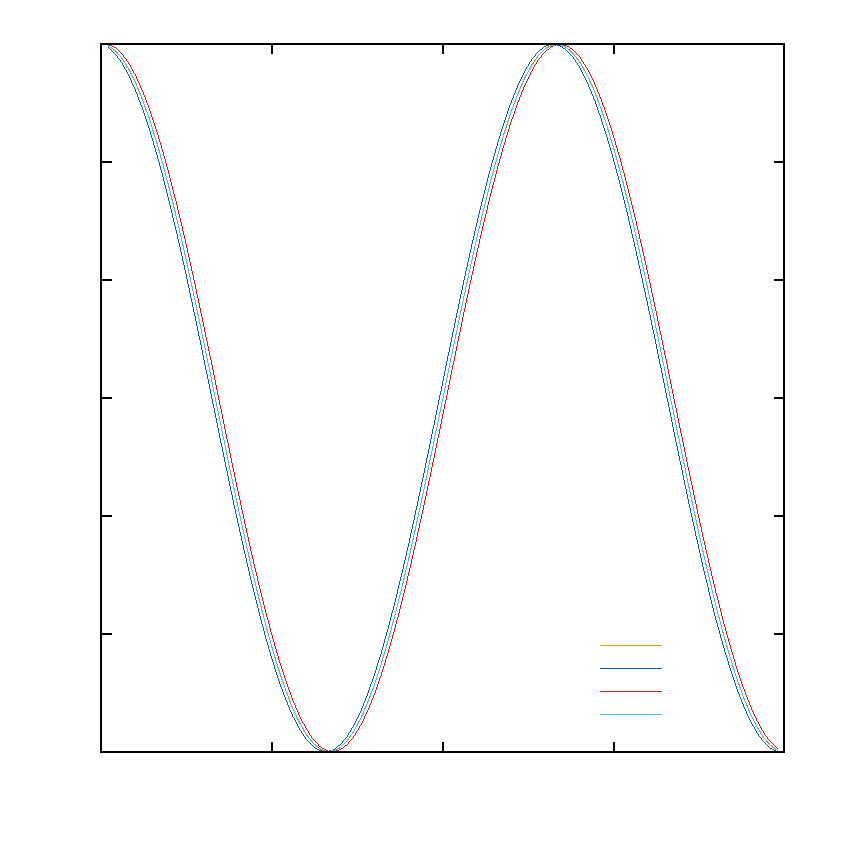
\includegraphics{D:/PhD/Tasks/004/report/firstsin100}}%
    \gplfronttext
  \end{picture}%
\endgroup

\caption{Comparison of numerical differentiation of sin$(3x)$ using 100
intervals for the first derivative}
\end{figure}

\section*{Numerical differentiation using arrays for the second
derivative}
C++ arrays were also used for numerical differentation of the second
derivative using schemes similar to those for first derivative. The function
sin$(3x)$ was differentiated twice using forward difference, backward difference
and central difference methods.

\subsection*{Forward difference method for second derivative}
\begin{equation}
f''(x) = \frac{f(x_{i+2})-2f(x_{i+1})+f(x_i)}{h^2}
\end{equation}

\subsection*{Backward difference method for second derivative}
\begin{equation}
f''(x) = \frac{f(x_i)-2f(x_{i-1})+f(x_{i-2})}{h^2}
\end{equation}

\subsection*{Central difference method for second derivative}
\begin{equation}
f''(x) = \frac{f(x_{i+1})-2f(x)+f(x_{i-1})}{h^2}
\end{equation}

The results for the second derivative are shown in the figures below.
\begin{figure}[p!]
\centering
% GNUPLOT: LaTeX picture with Postscript
\begingroup
  \makeatletter
  \providecommand\color[2][]{%
    \GenericError{(gnuplot) \space\space\space\@spaces}{%
      Package color not loaded in conjunction with
      terminal option `colourtext'%
    }{See the gnuplot documentation for explanation.%
    }{Either use 'blacktext' in gnuplot or load the package
      color.sty in LaTeX.}%
    \renewcommand\color[2][]{}%
  }%
  \providecommand\includegraphics[2][]{%
    \GenericError{(gnuplot) \space\space\space\@spaces}{%
      Package graphicx or graphics not loaded%
    }{See the gnuplot documentation for explanation.%
    }{The gnuplot epslatex terminal needs graphicx.sty or graphics.sty.}%
    \renewcommand\includegraphics[2][]{}%
  }%
  \providecommand\rotatebox[2]{#2}%
  \@ifundefined{ifGPcolor}{%
    \newif\ifGPcolor
    \GPcolortrue
  }{}%
  \@ifundefined{ifGPblacktext}{%
    \newif\ifGPblacktext
    \GPblacktextfalse
  }{}%
  % define a \g@addto@macro without @ in the name:
  \let\gplgaddtomacro\g@addto@macro
  % define empty templates for all commands taking text:
  \gdef\gplbacktext{}%
  \gdef\gplfronttext{}%
  \makeatother
  \ifGPblacktext
    % no textcolor at all
    \def\colorrgb#1{}%
    \def\colorgray#1{}%
  \else
    % gray or color?
    \ifGPcolor
      \def\colorrgb#1{\color[rgb]{#1}}%
      \def\colorgray#1{\color[gray]{#1}}%
      \expandafter\def\csname LTw\endcsname{\color{white}}%
      \expandafter\def\csname LTb\endcsname{\color{black}}%
      \expandafter\def\csname LTa\endcsname{\color{black}}%
      \expandafter\def\csname LT0\endcsname{\color[rgb]{1,0,0}}%
      \expandafter\def\csname LT1\endcsname{\color[rgb]{0,1,0}}%
      \expandafter\def\csname LT2\endcsname{\color[rgb]{0,0,1}}%
      \expandafter\def\csname LT3\endcsname{\color[rgb]{1,0,1}}%
      \expandafter\def\csname LT4\endcsname{\color[rgb]{0,1,1}}%
      \expandafter\def\csname LT5\endcsname{\color[rgb]{1,1,0}}%
      \expandafter\def\csname LT6\endcsname{\color[rgb]{0,0,0}}%
      \expandafter\def\csname LT7\endcsname{\color[rgb]{1,0.3,0}}%
      \expandafter\def\csname LT8\endcsname{\color[rgb]{0.5,0.5,0.5}}%
    \else
      % gray
      \def\colorrgb#1{\color{black}}%
      \def\colorgray#1{\color[gray]{#1}}%
      \expandafter\def\csname LTw\endcsname{\color{white}}%
      \expandafter\def\csname LTb\endcsname{\color{black}}%
      \expandafter\def\csname LTa\endcsname{\color{black}}%
      \expandafter\def\csname LT0\endcsname{\color{black}}%
      \expandafter\def\csname LT1\endcsname{\color{black}}%
      \expandafter\def\csname LT2\endcsname{\color{black}}%
      \expandafter\def\csname LT3\endcsname{\color{black}}%
      \expandafter\def\csname LT4\endcsname{\color{black}}%
      \expandafter\def\csname LT5\endcsname{\color{black}}%
      \expandafter\def\csname LT6\endcsname{\color{black}}%
      \expandafter\def\csname LT7\endcsname{\color{black}}%
      \expandafter\def\csname LT8\endcsname{\color{black}}%
    \fi
  \fi
    \setlength{\unitlength}{0.0500bp}%
    \ifx\gptboxheight\undefined%
      \newlength{\gptboxheight}%
      \newlength{\gptboxwidth}%
      \newsavebox{\gptboxtext}%
    \fi%
    \setlength{\fboxrule}{0.5pt}%
    \setlength{\fboxsep}{1pt}%
\begin{picture}(7766.00,7766.00)%
    \gplgaddtomacro\gplbacktext{%
      \csname LTb\endcsname%
      \put(814,704){\makebox(0,0)[r]{\strut{}$-10$}}%
      \put(814,1384){\makebox(0,0)[r]{\strut{}$-8$}}%
      \put(814,2063){\makebox(0,0)[r]{\strut{}$-6$}}%
      \put(814,2743){\makebox(0,0)[r]{\strut{}$-4$}}%
      \put(814,3423){\makebox(0,0)[r]{\strut{}$-2$}}%
      \put(814,4103){\makebox(0,0)[r]{\strut{}$0$}}%
      \put(814,4782){\makebox(0,0)[r]{\strut{}$2$}}%
      \put(814,5462){\makebox(0,0)[r]{\strut{}$4$}}%
      \put(814,6142){\makebox(0,0)[r]{\strut{}$6$}}%
      \put(814,6821){\makebox(0,0)[r]{\strut{}$8$}}%
      \put(814,7501){\makebox(0,0)[r]{\strut{}$10$}}%
      \put(946,484){\makebox(0,0){\strut{}$0$}}%
      \put(2552,484){\makebox(0,0){\strut{}$\pi/4$}}%
      \put(4158,484){\makebox(0,0){\strut{}$\pi/2$}}%
      \put(5763,484){\makebox(0,0){\strut{}$3\pi/4$}}%
      \put(7369,484){\makebox(0,0){\strut{}$\pi$}}%
    }%
    \gplgaddtomacro\gplfronttext{%
      \csname LTb\endcsname%
      \put(176,4102){\rotatebox{-270}{\makebox(0,0){\strut{}$f(x)$}}}%
      \put(4157,154){\makebox(0,0){\strut{}$x$}}%
      \csname LTb\endcsname%
      \put(6310,7051){\makebox(0,0)[r]{\strut{}Analytical}}%
      \csname LTb\endcsname%
      \put(6310,6831){\makebox(0,0)[r]{\strut{}Forward}}%
      \csname LTb\endcsname%
      \put(6310,6611){\makebox(0,0)[r]{\strut{}Backward}}%
      \csname LTb\endcsname%
      \put(6310,6391){\makebox(0,0)[r]{\strut{}Central}}%
    }%
    \gplbacktext
    \put(0,0){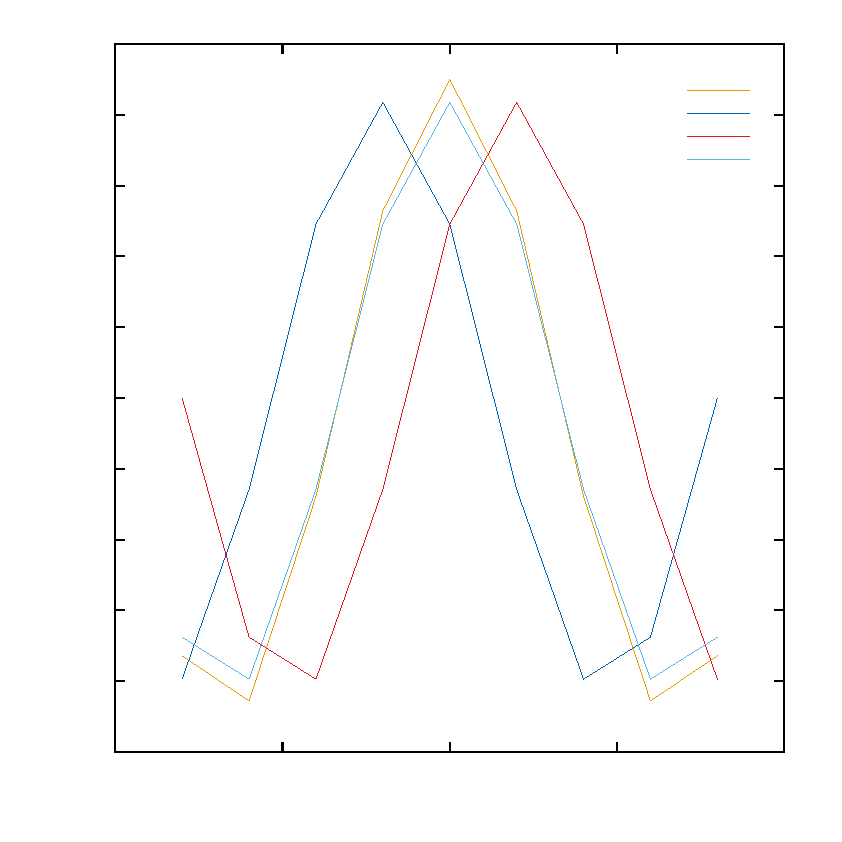
\includegraphics{D:/PhD/Tasks/004/report/secondsin10}}%
    \gplfronttext
  \end{picture}%
\endgroup

\caption{Comparison of numerical differentiation of second derivative
of sin$(3x)$ using 10 intervals}
\end{figure}
\begin{figure}[p!]
\centering
% GNUPLOT: LaTeX picture with Postscript
\begingroup
  \makeatletter
  \providecommand\color[2][]{%
    \GenericError{(gnuplot) \space\space\space\@spaces}{%
      Package color not loaded in conjunction with
      terminal option `colourtext'%
    }{See the gnuplot documentation for explanation.%
    }{Either use 'blacktext' in gnuplot or load the package
      color.sty in LaTeX.}%
    \renewcommand\color[2][]{}%
  }%
  \providecommand\includegraphics[2][]{%
    \GenericError{(gnuplot) \space\space\space\@spaces}{%
      Package graphicx or graphics not loaded%
    }{See the gnuplot documentation for explanation.%
    }{The gnuplot epslatex terminal needs graphicx.sty or graphics.sty.}%
    \renewcommand\includegraphics[2][]{}%
  }%
  \providecommand\rotatebox[2]{#2}%
  \@ifundefined{ifGPcolor}{%
    \newif\ifGPcolor
    \GPcolortrue
  }{}%
  \@ifundefined{ifGPblacktext}{%
    \newif\ifGPblacktext
    \GPblacktextfalse
  }{}%
  % define a \g@addto@macro without @ in the name:
  \let\gplgaddtomacro\g@addto@macro
  % define empty templates for all commands taking text:
  \gdef\gplbacktext{}%
  \gdef\gplfronttext{}%
  \makeatother
  \ifGPblacktext
    % no textcolor at all
    \def\colorrgb#1{}%
    \def\colorgray#1{}%
  \else
    % gray or color?
    \ifGPcolor
      \def\colorrgb#1{\color[rgb]{#1}}%
      \def\colorgray#1{\color[gray]{#1}}%
      \expandafter\def\csname LTw\endcsname{\color{white}}%
      \expandafter\def\csname LTb\endcsname{\color{black}}%
      \expandafter\def\csname LTa\endcsname{\color{black}}%
      \expandafter\def\csname LT0\endcsname{\color[rgb]{1,0,0}}%
      \expandafter\def\csname LT1\endcsname{\color[rgb]{0,1,0}}%
      \expandafter\def\csname LT2\endcsname{\color[rgb]{0,0,1}}%
      \expandafter\def\csname LT3\endcsname{\color[rgb]{1,0,1}}%
      \expandafter\def\csname LT4\endcsname{\color[rgb]{0,1,1}}%
      \expandafter\def\csname LT5\endcsname{\color[rgb]{1,1,0}}%
      \expandafter\def\csname LT6\endcsname{\color[rgb]{0,0,0}}%
      \expandafter\def\csname LT7\endcsname{\color[rgb]{1,0.3,0}}%
      \expandafter\def\csname LT8\endcsname{\color[rgb]{0.5,0.5,0.5}}%
    \else
      % gray
      \def\colorrgb#1{\color{black}}%
      \def\colorgray#1{\color[gray]{#1}}%
      \expandafter\def\csname LTw\endcsname{\color{white}}%
      \expandafter\def\csname LTb\endcsname{\color{black}}%
      \expandafter\def\csname LTa\endcsname{\color{black}}%
      \expandafter\def\csname LT0\endcsname{\color{black}}%
      \expandafter\def\csname LT1\endcsname{\color{black}}%
      \expandafter\def\csname LT2\endcsname{\color{black}}%
      \expandafter\def\csname LT3\endcsname{\color{black}}%
      \expandafter\def\csname LT4\endcsname{\color{black}}%
      \expandafter\def\csname LT5\endcsname{\color{black}}%
      \expandafter\def\csname LT6\endcsname{\color{black}}%
      \expandafter\def\csname LT7\endcsname{\color{black}}%
      \expandafter\def\csname LT8\endcsname{\color{black}}%
    \fi
  \fi
    \setlength{\unitlength}{0.0500bp}%
    \ifx\gptboxheight\undefined%
      \newlength{\gptboxheight}%
      \newlength{\gptboxwidth}%
      \newsavebox{\gptboxtext}%
    \fi%
    \setlength{\fboxrule}{0.5pt}%
    \setlength{\fboxsep}{1pt}%
\begin{picture}(7766.00,7766.00)%
    \gplgaddtomacro\gplbacktext{%
      \csname LTb\endcsname%
      \put(814,704){\makebox(0,0)[r]{\strut{}$-10$}}%
      \put(814,1384){\makebox(0,0)[r]{\strut{}$-8$}}%
      \put(814,2063){\makebox(0,0)[r]{\strut{}$-6$}}%
      \put(814,2743){\makebox(0,0)[r]{\strut{}$-4$}}%
      \put(814,3423){\makebox(0,0)[r]{\strut{}$-2$}}%
      \put(814,4103){\makebox(0,0)[r]{\strut{}$0$}}%
      \put(814,4782){\makebox(0,0)[r]{\strut{}$2$}}%
      \put(814,5462){\makebox(0,0)[r]{\strut{}$4$}}%
      \put(814,6142){\makebox(0,0)[r]{\strut{}$6$}}%
      \put(814,6821){\makebox(0,0)[r]{\strut{}$8$}}%
      \put(814,7501){\makebox(0,0)[r]{\strut{}$10$}}%
      \put(946,484){\makebox(0,0){\strut{}$0$}}%
      \put(2552,484){\makebox(0,0){\strut{}$\pi/4$}}%
      \put(4158,484){\makebox(0,0){\strut{}$\pi/2$}}%
      \put(5763,484){\makebox(0,0){\strut{}$3\pi/4$}}%
      \put(7369,484){\makebox(0,0){\strut{}$\pi$}}%
    }%
    \gplgaddtomacro\gplfronttext{%
      \csname LTb\endcsname%
      \put(176,4102){\rotatebox{-270}{\makebox(0,0){\strut{}$f(x)$}}}%
      \put(4157,154){\makebox(0,0){\strut{}$x$}}%
      \csname LTb\endcsname%
      \put(6310,7051){\makebox(0,0)[r]{\strut{}Analytical}}%
      \csname LTb\endcsname%
      \put(6310,6831){\makebox(0,0)[r]{\strut{}Forward}}%
      \csname LTb\endcsname%
      \put(6310,6611){\makebox(0,0)[r]{\strut{}Backward}}%
      \csname LTb\endcsname%
      \put(6310,6391){\makebox(0,0)[r]{\strut{}Central}}%
    }%
    \gplbacktext
    \put(0,0){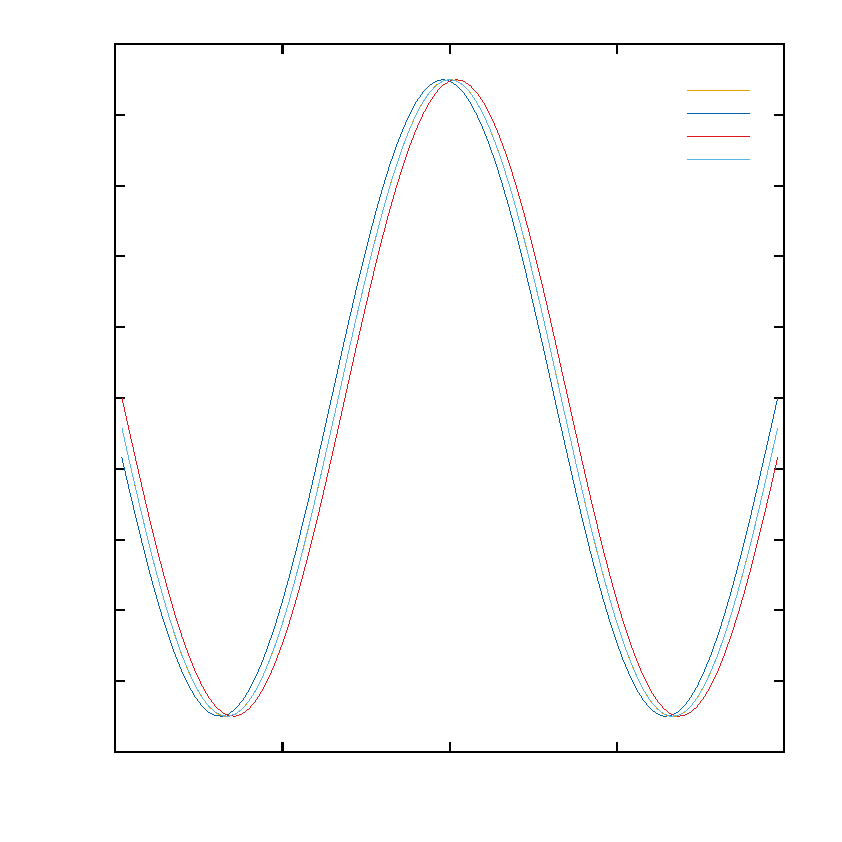
\includegraphics{D:/PhD/Tasks/004/report/secondsin100}}%
    \gplfronttext
  \end{picture}%
\endgroup

\caption{Comparison of numerical differentiation of second derivative
of sin$(3x)$ using 100 intervals}
\end{figure}

\newpage
\section*{Determination of error for for first and second derivatives}
The error for calculation of the first derivative was determined for
each of the three differnt methods using the following formula:
\begin{equation}
E = \sqrt{\frac{\sum\limits_{i=1}^{N}\left(\frac{A_N-A_a}{A_a}\right)^2}{N}}
\end{equation}
The calculations were performed for intervals starting from 10 to 10,000 over
the range 0 to $pi$. The plots are shown below.
\begin{figure}[p!]
\centering
% GNUPLOT: LaTeX picture with Postscript
\begingroup
  \makeatletter
  \providecommand\color[2][]{%
    \GenericError{(gnuplot) \space\space\space\@spaces}{%
      Package color not loaded in conjunction with
      terminal option `colourtext'%
    }{See the gnuplot documentation for explanation.%
    }{Either use 'blacktext' in gnuplot or load the package
      color.sty in LaTeX.}%
    \renewcommand\color[2][]{}%
  }%
  \providecommand\includegraphics[2][]{%
    \GenericError{(gnuplot) \space\space\space\@spaces}{%
      Package graphicx or graphics not loaded%
    }{See the gnuplot documentation for explanation.%
    }{The gnuplot epslatex terminal needs graphicx.sty or graphics.sty.}%
    \renewcommand\includegraphics[2][]{}%
  }%
  \providecommand\rotatebox[2]{#2}%
  \@ifundefined{ifGPcolor}{%
    \newif\ifGPcolor
    \GPcolortrue
  }{}%
  \@ifundefined{ifGPblacktext}{%
    \newif\ifGPblacktext
    \GPblacktextfalse
  }{}%
  % define a \g@addto@macro without @ in the name:
  \let\gplgaddtomacro\g@addto@macro
  % define empty templates for all commands taking text:
  \gdef\gplbacktext{}%
  \gdef\gplfronttext{}%
  \makeatother
  \ifGPblacktext
    % no textcolor at all
    \def\colorrgb#1{}%
    \def\colorgray#1{}%
  \else
    % gray or color?
    \ifGPcolor
      \def\colorrgb#1{\color[rgb]{#1}}%
      \def\colorgray#1{\color[gray]{#1}}%
      \expandafter\def\csname LTw\endcsname{\color{white}}%
      \expandafter\def\csname LTb\endcsname{\color{black}}%
      \expandafter\def\csname LTa\endcsname{\color{black}}%
      \expandafter\def\csname LT0\endcsname{\color[rgb]{1,0,0}}%
      \expandafter\def\csname LT1\endcsname{\color[rgb]{0,1,0}}%
      \expandafter\def\csname LT2\endcsname{\color[rgb]{0,0,1}}%
      \expandafter\def\csname LT3\endcsname{\color[rgb]{1,0,1}}%
      \expandafter\def\csname LT4\endcsname{\color[rgb]{0,1,1}}%
      \expandafter\def\csname LT5\endcsname{\color[rgb]{1,1,0}}%
      \expandafter\def\csname LT6\endcsname{\color[rgb]{0,0,0}}%
      \expandafter\def\csname LT7\endcsname{\color[rgb]{1,0.3,0}}%
      \expandafter\def\csname LT8\endcsname{\color[rgb]{0.5,0.5,0.5}}%
    \else
      % gray
      \def\colorrgb#1{\color{black}}%
      \def\colorgray#1{\color[gray]{#1}}%
      \expandafter\def\csname LTw\endcsname{\color{white}}%
      \expandafter\def\csname LTb\endcsname{\color{black}}%
      \expandafter\def\csname LTa\endcsname{\color{black}}%
      \expandafter\def\csname LT0\endcsname{\color{black}}%
      \expandafter\def\csname LT1\endcsname{\color{black}}%
      \expandafter\def\csname LT2\endcsname{\color{black}}%
      \expandafter\def\csname LT3\endcsname{\color{black}}%
      \expandafter\def\csname LT4\endcsname{\color{black}}%
      \expandafter\def\csname LT5\endcsname{\color{black}}%
      \expandafter\def\csname LT6\endcsname{\color{black}}%
      \expandafter\def\csname LT7\endcsname{\color{black}}%
      \expandafter\def\csname LT8\endcsname{\color{black}}%
    \fi
  \fi
    \setlength{\unitlength}{0.0500bp}%
    \ifx\gptboxheight\undefined%
      \newlength{\gptboxheight}%
      \newlength{\gptboxwidth}%
      \newsavebox{\gptboxtext}%
    \fi%
    \setlength{\fboxrule}{0.5pt}%
    \setlength{\fboxsep}{1pt}%
\begin{picture}(7766.00,7766.00)%
    \gplgaddtomacro\gplbacktext{%
      \csname LTb\endcsname%
      \put(682,704){\makebox(0,0)[r]{\strut{}$-2$}}%
      \put(682,1459){\makebox(0,0)[r]{\strut{}$0$}}%
      \put(682,2214){\makebox(0,0)[r]{\strut{}$2$}}%
      \put(682,2970){\makebox(0,0)[r]{\strut{}$4$}}%
      \put(682,3725){\makebox(0,0)[r]{\strut{}$6$}}%
      \put(682,4480){\makebox(0,0)[r]{\strut{}$8$}}%
      \put(682,5235){\makebox(0,0)[r]{\strut{}$10$}}%
      \put(682,5991){\makebox(0,0)[r]{\strut{}$12$}}%
      \put(682,6746){\makebox(0,0)[r]{\strut{}$14$}}%
      \put(682,7501){\makebox(0,0)[r]{\strut{}$16$}}%
      \put(814,484){\makebox(0,0){\strut{}$1$}}%
      \put(2453,484){\makebox(0,0){\strut{}$10$}}%
      \put(4092,484){\makebox(0,0){\strut{}$100$}}%
      \put(5730,484){\makebox(0,0){\strut{}$1000$}}%
      \put(7369,484){\makebox(0,0){\strut{}$10000$}}%
    }%
    \gplgaddtomacro\gplfronttext{%
      \csname LTb\endcsname%
      \put(176,4102){\rotatebox{-270}{\makebox(0,0){\strut{}log$_{10}E$}}}%
      \put(4091,154){\makebox(0,0){\strut{}log$_{10}N$}}%
    }%
    \gplbacktext
    \put(0,0){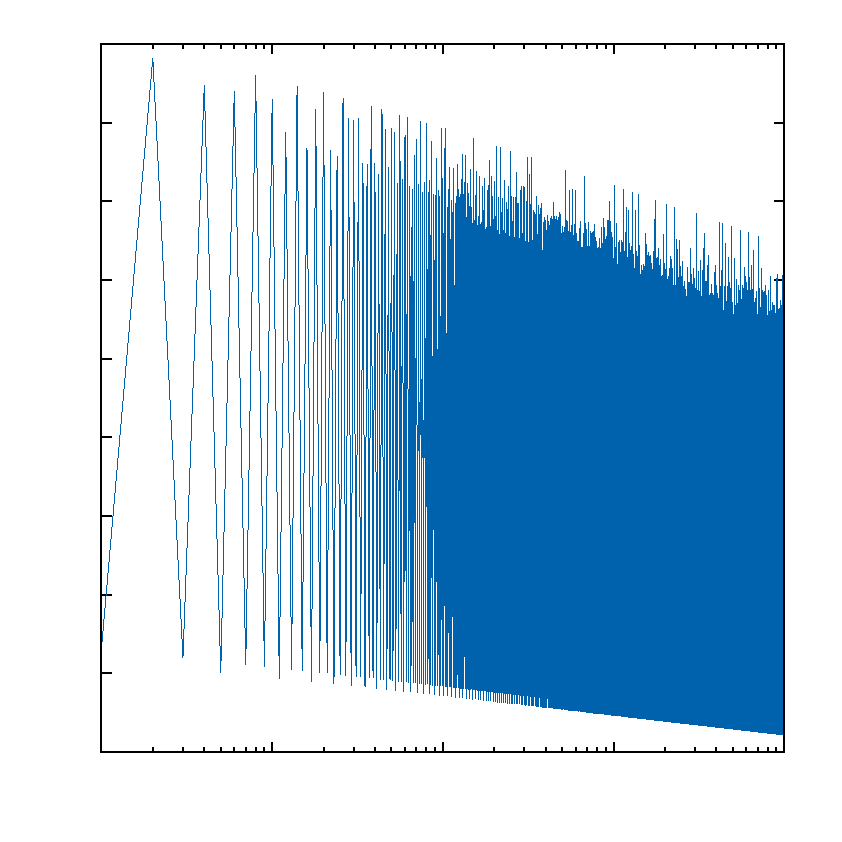
\includegraphics{D:/PhD/Tasks/004/report/firstsinfwderror}}%
    \gplfronttext
  \end{picture}%
\endgroup

\caption{Plot of log\textsubscript{10}$E$ versus log\textsubscript{10}$N$ for
numerical differentiation of first derivative using forward difference method}
\end{figure}
\begin{figure}[p!]
\centering
% GNUPLOT: LaTeX picture with Postscript
\begingroup
  \makeatletter
  \providecommand\color[2][]{%
    \GenericError{(gnuplot) \space\space\space\@spaces}{%
      Package color not loaded in conjunction with
      terminal option `colourtext'%
    }{See the gnuplot documentation for explanation.%
    }{Either use 'blacktext' in gnuplot or load the package
      color.sty in LaTeX.}%
    \renewcommand\color[2][]{}%
  }%
  \providecommand\includegraphics[2][]{%
    \GenericError{(gnuplot) \space\space\space\@spaces}{%
      Package graphicx or graphics not loaded%
    }{See the gnuplot documentation for explanation.%
    }{The gnuplot epslatex terminal needs graphicx.sty or graphics.sty.}%
    \renewcommand\includegraphics[2][]{}%
  }%
  \providecommand\rotatebox[2]{#2}%
  \@ifundefined{ifGPcolor}{%
    \newif\ifGPcolor
    \GPcolortrue
  }{}%
  \@ifundefined{ifGPblacktext}{%
    \newif\ifGPblacktext
    \GPblacktextfalse
  }{}%
  % define a \g@addto@macro without @ in the name:
  \let\gplgaddtomacro\g@addto@macro
  % define empty templates for all commands taking text:
  \gdef\gplbacktext{}%
  \gdef\gplfronttext{}%
  \makeatother
  \ifGPblacktext
    % no textcolor at all
    \def\colorrgb#1{}%
    \def\colorgray#1{}%
  \else
    % gray or color?
    \ifGPcolor
      \def\colorrgb#1{\color[rgb]{#1}}%
      \def\colorgray#1{\color[gray]{#1}}%
      \expandafter\def\csname LTw\endcsname{\color{white}}%
      \expandafter\def\csname LTb\endcsname{\color{black}}%
      \expandafter\def\csname LTa\endcsname{\color{black}}%
      \expandafter\def\csname LT0\endcsname{\color[rgb]{1,0,0}}%
      \expandafter\def\csname LT1\endcsname{\color[rgb]{0,1,0}}%
      \expandafter\def\csname LT2\endcsname{\color[rgb]{0,0,1}}%
      \expandafter\def\csname LT3\endcsname{\color[rgb]{1,0,1}}%
      \expandafter\def\csname LT4\endcsname{\color[rgb]{0,1,1}}%
      \expandafter\def\csname LT5\endcsname{\color[rgb]{1,1,0}}%
      \expandafter\def\csname LT6\endcsname{\color[rgb]{0,0,0}}%
      \expandafter\def\csname LT7\endcsname{\color[rgb]{1,0.3,0}}%
      \expandafter\def\csname LT8\endcsname{\color[rgb]{0.5,0.5,0.5}}%
    \else
      % gray
      \def\colorrgb#1{\color{black}}%
      \def\colorgray#1{\color[gray]{#1}}%
      \expandafter\def\csname LTw\endcsname{\color{white}}%
      \expandafter\def\csname LTb\endcsname{\color{black}}%
      \expandafter\def\csname LTa\endcsname{\color{black}}%
      \expandafter\def\csname LT0\endcsname{\color{black}}%
      \expandafter\def\csname LT1\endcsname{\color{black}}%
      \expandafter\def\csname LT2\endcsname{\color{black}}%
      \expandafter\def\csname LT3\endcsname{\color{black}}%
      \expandafter\def\csname LT4\endcsname{\color{black}}%
      \expandafter\def\csname LT5\endcsname{\color{black}}%
      \expandafter\def\csname LT6\endcsname{\color{black}}%
      \expandafter\def\csname LT7\endcsname{\color{black}}%
      \expandafter\def\csname LT8\endcsname{\color{black}}%
    \fi
  \fi
    \setlength{\unitlength}{0.0500bp}%
    \ifx\gptboxheight\undefined%
      \newlength{\gptboxheight}%
      \newlength{\gptboxwidth}%
      \newsavebox{\gptboxtext}%
    \fi%
    \setlength{\fboxrule}{0.5pt}%
    \setlength{\fboxsep}{1pt}%
\begin{picture}(7766.00,7766.00)%
    \gplgaddtomacro\gplbacktext{%
      \csname LTb\endcsname%
      \put(682,704){\makebox(0,0)[r]{\strut{}$0$}}%
      \put(682,1384){\makebox(0,0)[r]{\strut{}$5$}}%
      \put(682,2063){\makebox(0,0)[r]{\strut{}$10$}}%
      \put(682,2743){\makebox(0,0)[r]{\strut{}$15$}}%
      \put(682,3423){\makebox(0,0)[r]{\strut{}$20$}}%
      \put(682,4102){\makebox(0,0)[r]{\strut{}$25$}}%
      \put(682,4782){\makebox(0,0)[r]{\strut{}$30$}}%
      \put(682,5462){\makebox(0,0)[r]{\strut{}$35$}}%
      \put(682,6142){\makebox(0,0)[r]{\strut{}$40$}}%
      \put(682,6821){\makebox(0,0)[r]{\strut{}$45$}}%
      \put(682,7501){\makebox(0,0)[r]{\strut{}$50$}}%
      \put(814,484){\makebox(0,0){\strut{}$1$}}%
      \put(2453,484){\makebox(0,0){\strut{}$10$}}%
      \put(4092,484){\makebox(0,0){\strut{}$100$}}%
      \put(5730,484){\makebox(0,0){\strut{}$1000$}}%
      \put(7369,484){\makebox(0,0){\strut{}$10000$}}%
    }%
    \gplgaddtomacro\gplfronttext{%
      \csname LTb\endcsname%
      \put(176,4102){\rotatebox{-270}{\makebox(0,0){\strut{}log$_{10}E$}}}%
      \put(4091,154){\makebox(0,0){\strut{}log$_{10}N$}}%
    }%
    \gplbacktext
    \put(0,0){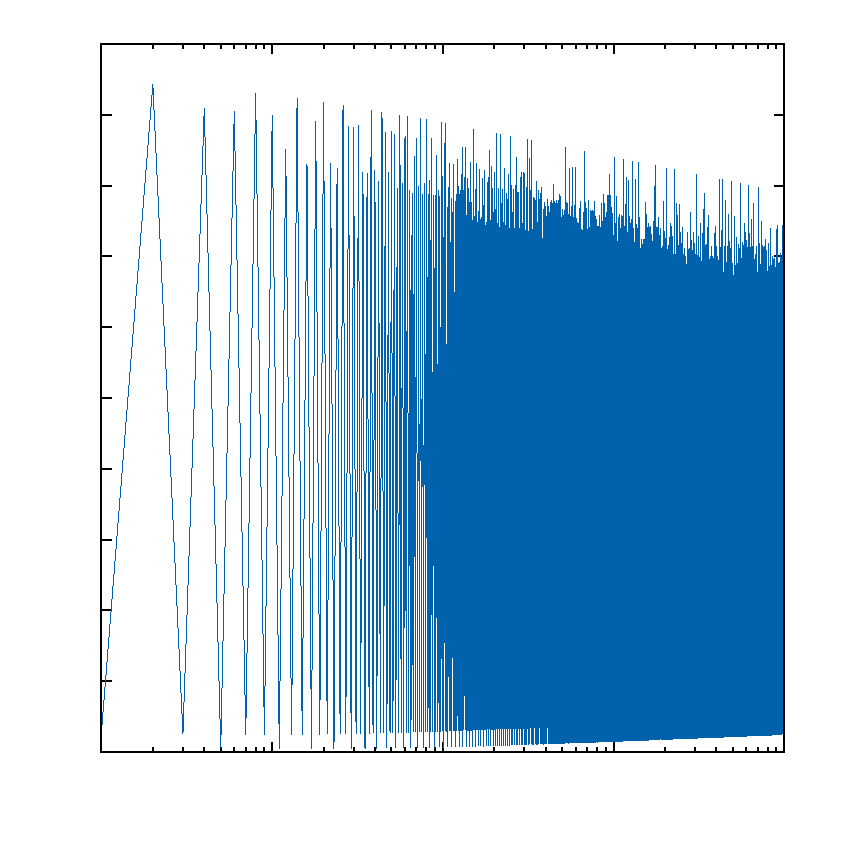
\includegraphics{D:/PhD/Tasks/004/report/firstsinbwderror}}%
    \gplfronttext
  \end{picture}%
\endgroup

\caption{Plot of log\textsubscript{10}$E$ versus log\textsubscript{10}$N$ for
numerical differentiation of first derivative using backward difference method}
\end{figure}
\begin{figure}[p!]
\centering
% GNUPLOT: LaTeX picture with Postscript
\begingroup
  \makeatletter
  \providecommand\color[2][]{%
    \GenericError{(gnuplot) \space\space\space\@spaces}{%
      Package color not loaded in conjunction with
      terminal option `colourtext'%
    }{See the gnuplot documentation for explanation.%
    }{Either use 'blacktext' in gnuplot or load the package
      color.sty in LaTeX.}%
    \renewcommand\color[2][]{}%
  }%
  \providecommand\includegraphics[2][]{%
    \GenericError{(gnuplot) \space\space\space\@spaces}{%
      Package graphicx or graphics not loaded%
    }{See the gnuplot documentation for explanation.%
    }{The gnuplot epslatex terminal needs graphicx.sty or graphics.sty.}%
    \renewcommand\includegraphics[2][]{}%
  }%
  \providecommand\rotatebox[2]{#2}%
  \@ifundefined{ifGPcolor}{%
    \newif\ifGPcolor
    \GPcolortrue
  }{}%
  \@ifundefined{ifGPblacktext}{%
    \newif\ifGPblacktext
    \GPblacktextfalse
  }{}%
  % define a \g@addto@macro without @ in the name:
  \let\gplgaddtomacro\g@addto@macro
  % define empty templates for all commands taking text:
  \gdef\gplbacktext{}%
  \gdef\gplfronttext{}%
  \makeatother
  \ifGPblacktext
    % no textcolor at all
    \def\colorrgb#1{}%
    \def\colorgray#1{}%
  \else
    % gray or color?
    \ifGPcolor
      \def\colorrgb#1{\color[rgb]{#1}}%
      \def\colorgray#1{\color[gray]{#1}}%
      \expandafter\def\csname LTw\endcsname{\color{white}}%
      \expandafter\def\csname LTb\endcsname{\color{black}}%
      \expandafter\def\csname LTa\endcsname{\color{black}}%
      \expandafter\def\csname LT0\endcsname{\color[rgb]{1,0,0}}%
      \expandafter\def\csname LT1\endcsname{\color[rgb]{0,1,0}}%
      \expandafter\def\csname LT2\endcsname{\color[rgb]{0,0,1}}%
      \expandafter\def\csname LT3\endcsname{\color[rgb]{1,0,1}}%
      \expandafter\def\csname LT4\endcsname{\color[rgb]{0,1,1}}%
      \expandafter\def\csname LT5\endcsname{\color[rgb]{1,1,0}}%
      \expandafter\def\csname LT6\endcsname{\color[rgb]{0,0,0}}%
      \expandafter\def\csname LT7\endcsname{\color[rgb]{1,0.3,0}}%
      \expandafter\def\csname LT8\endcsname{\color[rgb]{0.5,0.5,0.5}}%
    \else
      % gray
      \def\colorrgb#1{\color{black}}%
      \def\colorgray#1{\color[gray]{#1}}%
      \expandafter\def\csname LTw\endcsname{\color{white}}%
      \expandafter\def\csname LTb\endcsname{\color{black}}%
      \expandafter\def\csname LTa\endcsname{\color{black}}%
      \expandafter\def\csname LT0\endcsname{\color{black}}%
      \expandafter\def\csname LT1\endcsname{\color{black}}%
      \expandafter\def\csname LT2\endcsname{\color{black}}%
      \expandafter\def\csname LT3\endcsname{\color{black}}%
      \expandafter\def\csname LT4\endcsname{\color{black}}%
      \expandafter\def\csname LT5\endcsname{\color{black}}%
      \expandafter\def\csname LT6\endcsname{\color{black}}%
      \expandafter\def\csname LT7\endcsname{\color{black}}%
      \expandafter\def\csname LT8\endcsname{\color{black}}%
    \fi
  \fi
    \setlength{\unitlength}{0.0500bp}%
    \ifx\gptboxheight\undefined%
      \newlength{\gptboxheight}%
      \newlength{\gptboxwidth}%
      \newsavebox{\gptboxtext}%
    \fi%
    \setlength{\fboxrule}{0.5pt}%
    \setlength{\fboxsep}{1pt}%
\begin{picture}(7766.00,7766.00)%
    \gplgaddtomacro\gplbacktext{%
      \csname LTb\endcsname%
      \put(682,704){\makebox(0,0)[r]{\strut{}$0$}}%
      \put(682,1384){\makebox(0,0)[r]{\strut{}$5$}}%
      \put(682,2063){\makebox(0,0)[r]{\strut{}$10$}}%
      \put(682,2743){\makebox(0,0)[r]{\strut{}$15$}}%
      \put(682,3423){\makebox(0,0)[r]{\strut{}$20$}}%
      \put(682,4102){\makebox(0,0)[r]{\strut{}$25$}}%
      \put(682,4782){\makebox(0,0)[r]{\strut{}$30$}}%
      \put(682,5462){\makebox(0,0)[r]{\strut{}$35$}}%
      \put(682,6142){\makebox(0,0)[r]{\strut{}$40$}}%
      \put(682,6821){\makebox(0,0)[r]{\strut{}$45$}}%
      \put(682,7501){\makebox(0,0)[r]{\strut{}$50$}}%
      \put(814,484){\makebox(0,0){\strut{}$1$}}%
      \put(2453,484){\makebox(0,0){\strut{}$10$}}%
      \put(4092,484){\makebox(0,0){\strut{}$100$}}%
      \put(5730,484){\makebox(0,0){\strut{}$1000$}}%
      \put(7369,484){\makebox(0,0){\strut{}$10000$}}%
    }%
    \gplgaddtomacro\gplfronttext{%
      \csname LTb\endcsname%
      \put(176,4102){\rotatebox{-270}{\makebox(0,0){\strut{}log$_{10}E$}}}%
      \put(4091,154){\makebox(0,0){\strut{}log$_{10}N$}}%
    }%
    \gplbacktext
    \put(0,0){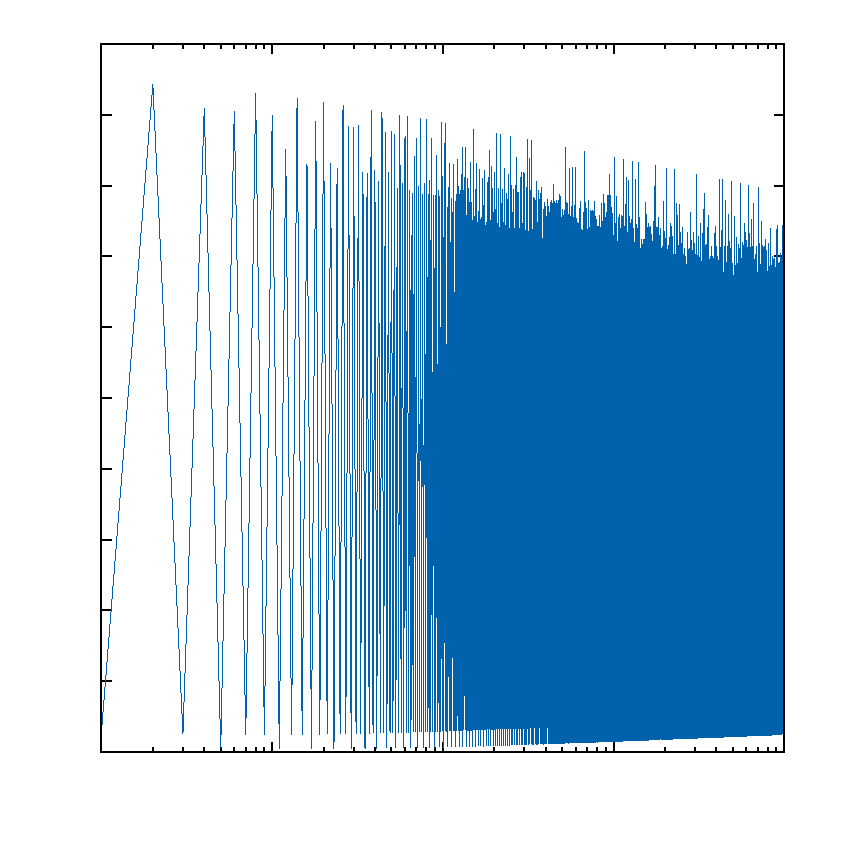
\includegraphics{D:/PhD/Tasks/004/report/firstsincnterror}}%
    \gplfronttext
  \end{picture}%
\endgroup

\caption{Plot of log\textsubscript{10}$E$ versus log\textsubscript{10}$N$ for
numerical differentiation of first derivative using central difference method}
\end{figure}

The error for calculation of the second derivative was also determined for
each of the three differnt methods using the same formula. The plot are as
follows.
\begin{figure}[p!]
\centering
% GNUPLOT: LaTeX picture with Postscript
\begingroup
  \makeatletter
  \providecommand\color[2][]{%
    \GenericError{(gnuplot) \space\space\space\@spaces}{%
      Package color not loaded in conjunction with
      terminal option `colourtext'%
    }{See the gnuplot documentation for explanation.%
    }{Either use 'blacktext' in gnuplot or load the package
      color.sty in LaTeX.}%
    \renewcommand\color[2][]{}%
  }%
  \providecommand\includegraphics[2][]{%
    \GenericError{(gnuplot) \space\space\space\@spaces}{%
      Package graphicx or graphics not loaded%
    }{See the gnuplot documentation for explanation.%
    }{The gnuplot epslatex terminal needs graphicx.sty or graphics.sty.}%
    \renewcommand\includegraphics[2][]{}%
  }%
  \providecommand\rotatebox[2]{#2}%
  \@ifundefined{ifGPcolor}{%
    \newif\ifGPcolor
    \GPcolortrue
  }{}%
  \@ifundefined{ifGPblacktext}{%
    \newif\ifGPblacktext
    \GPblacktextfalse
  }{}%
  % define a \g@addto@macro without @ in the name:
  \let\gplgaddtomacro\g@addto@macro
  % define empty templates for all commands taking text:
  \gdef\gplbacktext{}%
  \gdef\gplfronttext{}%
  \makeatother
  \ifGPblacktext
    % no textcolor at all
    \def\colorrgb#1{}%
    \def\colorgray#1{}%
  \else
    % gray or color?
    \ifGPcolor
      \def\colorrgb#1{\color[rgb]{#1}}%
      \def\colorgray#1{\color[gray]{#1}}%
      \expandafter\def\csname LTw\endcsname{\color{white}}%
      \expandafter\def\csname LTb\endcsname{\color{black}}%
      \expandafter\def\csname LTa\endcsname{\color{black}}%
      \expandafter\def\csname LT0\endcsname{\color[rgb]{1,0,0}}%
      \expandafter\def\csname LT1\endcsname{\color[rgb]{0,1,0}}%
      \expandafter\def\csname LT2\endcsname{\color[rgb]{0,0,1}}%
      \expandafter\def\csname LT3\endcsname{\color[rgb]{1,0,1}}%
      \expandafter\def\csname LT4\endcsname{\color[rgb]{0,1,1}}%
      \expandafter\def\csname LT5\endcsname{\color[rgb]{1,1,0}}%
      \expandafter\def\csname LT6\endcsname{\color[rgb]{0,0,0}}%
      \expandafter\def\csname LT7\endcsname{\color[rgb]{1,0.3,0}}%
      \expandafter\def\csname LT8\endcsname{\color[rgb]{0.5,0.5,0.5}}%
    \else
      % gray
      \def\colorrgb#1{\color{black}}%
      \def\colorgray#1{\color[gray]{#1}}%
      \expandafter\def\csname LTw\endcsname{\color{white}}%
      \expandafter\def\csname LTb\endcsname{\color{black}}%
      \expandafter\def\csname LTa\endcsname{\color{black}}%
      \expandafter\def\csname LT0\endcsname{\color{black}}%
      \expandafter\def\csname LT1\endcsname{\color{black}}%
      \expandafter\def\csname LT2\endcsname{\color{black}}%
      \expandafter\def\csname LT3\endcsname{\color{black}}%
      \expandafter\def\csname LT4\endcsname{\color{black}}%
      \expandafter\def\csname LT5\endcsname{\color{black}}%
      \expandafter\def\csname LT6\endcsname{\color{black}}%
      \expandafter\def\csname LT7\endcsname{\color{black}}%
      \expandafter\def\csname LT8\endcsname{\color{black}}%
    \fi
  \fi
    \setlength{\unitlength}{0.0500bp}%
    \ifx\gptboxheight\undefined%
      \newlength{\gptboxheight}%
      \newlength{\gptboxwidth}%
      \newsavebox{\gptboxtext}%
    \fi%
    \setlength{\fboxrule}{0.5pt}%
    \setlength{\fboxsep}{1pt}%
\begin{picture}(7766.00,7766.00)%
    \gplgaddtomacro\gplbacktext{%
      \csname LTb\endcsname%
      \put(682,704){\makebox(0,0)[r]{\strut{}$-2$}}%
      \put(682,1459){\makebox(0,0)[r]{\strut{}$0$}}%
      \put(682,2214){\makebox(0,0)[r]{\strut{}$2$}}%
      \put(682,2970){\makebox(0,0)[r]{\strut{}$4$}}%
      \put(682,3725){\makebox(0,0)[r]{\strut{}$6$}}%
      \put(682,4480){\makebox(0,0)[r]{\strut{}$8$}}%
      \put(682,5235){\makebox(0,0)[r]{\strut{}$10$}}%
      \put(682,5991){\makebox(0,0)[r]{\strut{}$12$}}%
      \put(682,6746){\makebox(0,0)[r]{\strut{}$14$}}%
      \put(682,7501){\makebox(0,0)[r]{\strut{}$16$}}%
      \put(814,484){\makebox(0,0){\strut{}$1$}}%
      \put(2453,484){\makebox(0,0){\strut{}$10$}}%
      \put(4092,484){\makebox(0,0){\strut{}$100$}}%
      \put(5730,484){\makebox(0,0){\strut{}$1000$}}%
      \put(7369,484){\makebox(0,0){\strut{}$10000$}}%
    }%
    \gplgaddtomacro\gplfronttext{%
      \csname LTb\endcsname%
      \put(176,4102){\rotatebox{-270}{\makebox(0,0){\strut{}log$_{10}E$}}}%
      \put(4091,154){\makebox(0,0){\strut{}log$_{10}N$}}%
    }%
    \gplbacktext
    \put(0,0){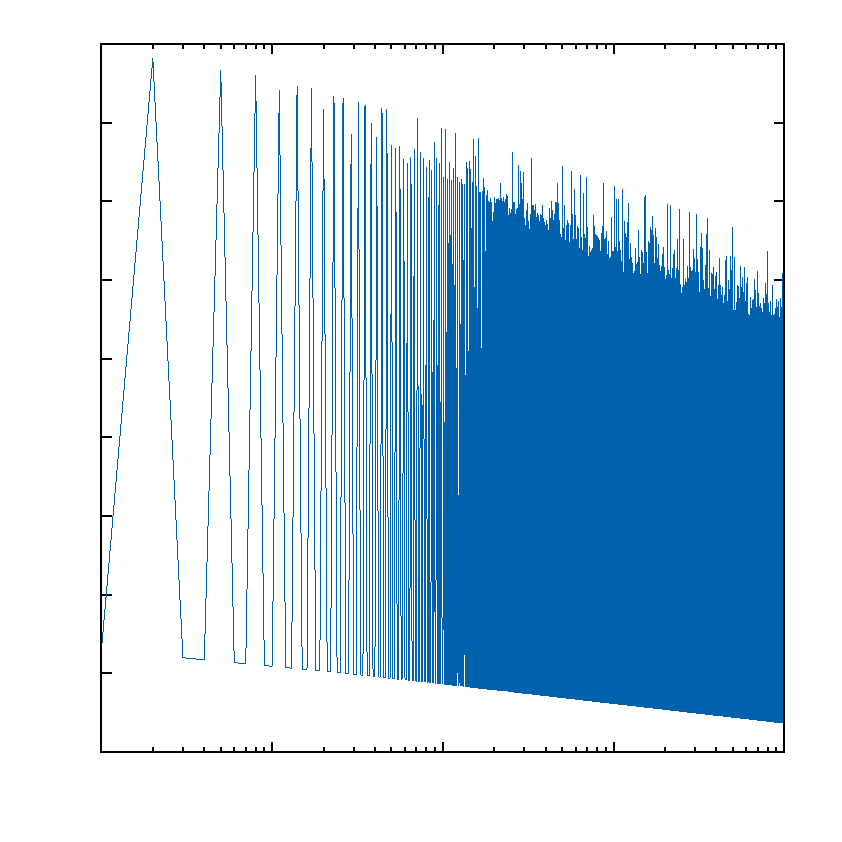
\includegraphics{D:/PhD/Tasks/004/report/secondsinfwderror}}%
    \gplfronttext
  \end{picture}%
\endgroup

\caption{Plot of log\textsubscript{10}$E$ versus log\textsubscript{10}$N$ for
numerical differentiation of second derivative using forward difference method}
\end{figure}
\begin{figure}[p!]
\centering
% GNUPLOT: LaTeX picture with Postscript
\begingroup
  \makeatletter
  \providecommand\color[2][]{%
    \GenericError{(gnuplot) \space\space\space\@spaces}{%
      Package color not loaded in conjunction with
      terminal option `colourtext'%
    }{See the gnuplot documentation for explanation.%
    }{Either use 'blacktext' in gnuplot or load the package
      color.sty in LaTeX.}%
    \renewcommand\color[2][]{}%
  }%
  \providecommand\includegraphics[2][]{%
    \GenericError{(gnuplot) \space\space\space\@spaces}{%
      Package graphicx or graphics not loaded%
    }{See the gnuplot documentation for explanation.%
    }{The gnuplot epslatex terminal needs graphicx.sty or graphics.sty.}%
    \renewcommand\includegraphics[2][]{}%
  }%
  \providecommand\rotatebox[2]{#2}%
  \@ifundefined{ifGPcolor}{%
    \newif\ifGPcolor
    \GPcolortrue
  }{}%
  \@ifundefined{ifGPblacktext}{%
    \newif\ifGPblacktext
    \GPblacktextfalse
  }{}%
  % define a \g@addto@macro without @ in the name:
  \let\gplgaddtomacro\g@addto@macro
  % define empty templates for all commands taking text:
  \gdef\gplbacktext{}%
  \gdef\gplfronttext{}%
  \makeatother
  \ifGPblacktext
    % no textcolor at all
    \def\colorrgb#1{}%
    \def\colorgray#1{}%
  \else
    % gray or color?
    \ifGPcolor
      \def\colorrgb#1{\color[rgb]{#1}}%
      \def\colorgray#1{\color[gray]{#1}}%
      \expandafter\def\csname LTw\endcsname{\color{white}}%
      \expandafter\def\csname LTb\endcsname{\color{black}}%
      \expandafter\def\csname LTa\endcsname{\color{black}}%
      \expandafter\def\csname LT0\endcsname{\color[rgb]{1,0,0}}%
      \expandafter\def\csname LT1\endcsname{\color[rgb]{0,1,0}}%
      \expandafter\def\csname LT2\endcsname{\color[rgb]{0,0,1}}%
      \expandafter\def\csname LT3\endcsname{\color[rgb]{1,0,1}}%
      \expandafter\def\csname LT4\endcsname{\color[rgb]{0,1,1}}%
      \expandafter\def\csname LT5\endcsname{\color[rgb]{1,1,0}}%
      \expandafter\def\csname LT6\endcsname{\color[rgb]{0,0,0}}%
      \expandafter\def\csname LT7\endcsname{\color[rgb]{1,0.3,0}}%
      \expandafter\def\csname LT8\endcsname{\color[rgb]{0.5,0.5,0.5}}%
    \else
      % gray
      \def\colorrgb#1{\color{black}}%
      \def\colorgray#1{\color[gray]{#1}}%
      \expandafter\def\csname LTw\endcsname{\color{white}}%
      \expandafter\def\csname LTb\endcsname{\color{black}}%
      \expandafter\def\csname LTa\endcsname{\color{black}}%
      \expandafter\def\csname LT0\endcsname{\color{black}}%
      \expandafter\def\csname LT1\endcsname{\color{black}}%
      \expandafter\def\csname LT2\endcsname{\color{black}}%
      \expandafter\def\csname LT3\endcsname{\color{black}}%
      \expandafter\def\csname LT4\endcsname{\color{black}}%
      \expandafter\def\csname LT5\endcsname{\color{black}}%
      \expandafter\def\csname LT6\endcsname{\color{black}}%
      \expandafter\def\csname LT7\endcsname{\color{black}}%
      \expandafter\def\csname LT8\endcsname{\color{black}}%
    \fi
  \fi
    \setlength{\unitlength}{0.0500bp}%
    \ifx\gptboxheight\undefined%
      \newlength{\gptboxheight}%
      \newlength{\gptboxwidth}%
      \newsavebox{\gptboxtext}%
    \fi%
    \setlength{\fboxrule}{0.5pt}%
    \setlength{\fboxsep}{1pt}%
\begin{picture}(7766.00,7766.00)%
    \gplgaddtomacro\gplbacktext{%
      \csname LTb\endcsname%
      \put(682,704){\makebox(0,0)[r]{\strut{}$0$}}%
      \put(682,1384){\makebox(0,0)[r]{\strut{}$5$}}%
      \put(682,2063){\makebox(0,0)[r]{\strut{}$10$}}%
      \put(682,2743){\makebox(0,0)[r]{\strut{}$15$}}%
      \put(682,3423){\makebox(0,0)[r]{\strut{}$20$}}%
      \put(682,4102){\makebox(0,0)[r]{\strut{}$25$}}%
      \put(682,4782){\makebox(0,0)[r]{\strut{}$30$}}%
      \put(682,5462){\makebox(0,0)[r]{\strut{}$35$}}%
      \put(682,6142){\makebox(0,0)[r]{\strut{}$40$}}%
      \put(682,6821){\makebox(0,0)[r]{\strut{}$45$}}%
      \put(682,7501){\makebox(0,0)[r]{\strut{}$50$}}%
      \put(814,484){\makebox(0,0){\strut{}$1$}}%
      \put(2453,484){\makebox(0,0){\strut{}$10$}}%
      \put(4092,484){\makebox(0,0){\strut{}$100$}}%
      \put(5730,484){\makebox(0,0){\strut{}$1000$}}%
      \put(7369,484){\makebox(0,0){\strut{}$10000$}}%
    }%
    \gplgaddtomacro\gplfronttext{%
      \csname LTb\endcsname%
      \put(176,4102){\rotatebox{-270}{\makebox(0,0){\strut{}log$_{10}E$}}}%
      \put(4091,154){\makebox(0,0){\strut{}log$_{10}N$}}%
    }%
    \gplbacktext
    \put(0,0){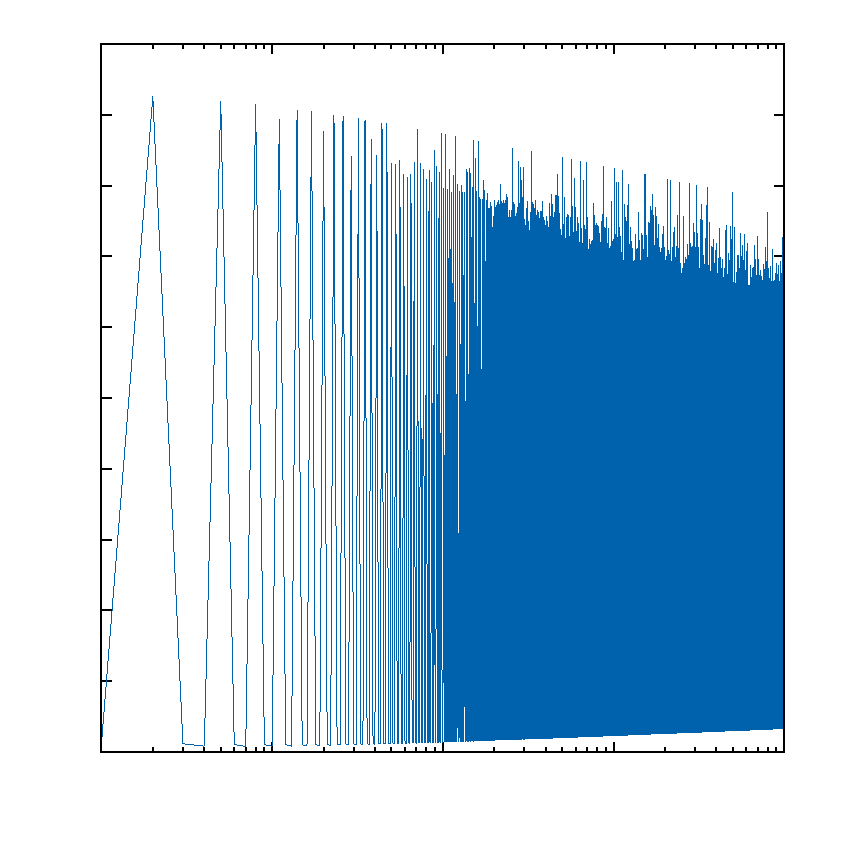
\includegraphics{D:/PhD/Tasks/004/report/secondsinbwderror}}%
    \gplfronttext
  \end{picture}%
\endgroup

\caption{Plot of log\textsubscript{10}$E$ versus log\textsubscript{10}$N$ for
numerical differentiation of second derivative using backward difference method}
\end{figure}
\begin{figure}[p!]
\centering
% GNUPLOT: LaTeX picture with Postscript
\begingroup
  \makeatletter
  \providecommand\color[2][]{%
    \GenericError{(gnuplot) \space\space\space\@spaces}{%
      Package color not loaded in conjunction with
      terminal option `colourtext'%
    }{See the gnuplot documentation for explanation.%
    }{Either use 'blacktext' in gnuplot or load the package
      color.sty in LaTeX.}%
    \renewcommand\color[2][]{}%
  }%
  \providecommand\includegraphics[2][]{%
    \GenericError{(gnuplot) \space\space\space\@spaces}{%
      Package graphicx or graphics not loaded%
    }{See the gnuplot documentation for explanation.%
    }{The gnuplot epslatex terminal needs graphicx.sty or graphics.sty.}%
    \renewcommand\includegraphics[2][]{}%
  }%
  \providecommand\rotatebox[2]{#2}%
  \@ifundefined{ifGPcolor}{%
    \newif\ifGPcolor
    \GPcolortrue
  }{}%
  \@ifundefined{ifGPblacktext}{%
    \newif\ifGPblacktext
    \GPblacktextfalse
  }{}%
  % define a \g@addto@macro without @ in the name:
  \let\gplgaddtomacro\g@addto@macro
  % define empty templates for all commands taking text:
  \gdef\gplbacktext{}%
  \gdef\gplfronttext{}%
  \makeatother
  \ifGPblacktext
    % no textcolor at all
    \def\colorrgb#1{}%
    \def\colorgray#1{}%
  \else
    % gray or color?
    \ifGPcolor
      \def\colorrgb#1{\color[rgb]{#1}}%
      \def\colorgray#1{\color[gray]{#1}}%
      \expandafter\def\csname LTw\endcsname{\color{white}}%
      \expandafter\def\csname LTb\endcsname{\color{black}}%
      \expandafter\def\csname LTa\endcsname{\color{black}}%
      \expandafter\def\csname LT0\endcsname{\color[rgb]{1,0,0}}%
      \expandafter\def\csname LT1\endcsname{\color[rgb]{0,1,0}}%
      \expandafter\def\csname LT2\endcsname{\color[rgb]{0,0,1}}%
      \expandafter\def\csname LT3\endcsname{\color[rgb]{1,0,1}}%
      \expandafter\def\csname LT4\endcsname{\color[rgb]{0,1,1}}%
      \expandafter\def\csname LT5\endcsname{\color[rgb]{1,1,0}}%
      \expandafter\def\csname LT6\endcsname{\color[rgb]{0,0,0}}%
      \expandafter\def\csname LT7\endcsname{\color[rgb]{1,0.3,0}}%
      \expandafter\def\csname LT8\endcsname{\color[rgb]{0.5,0.5,0.5}}%
    \else
      % gray
      \def\colorrgb#1{\color{black}}%
      \def\colorgray#1{\color[gray]{#1}}%
      \expandafter\def\csname LTw\endcsname{\color{white}}%
      \expandafter\def\csname LTb\endcsname{\color{black}}%
      \expandafter\def\csname LTa\endcsname{\color{black}}%
      \expandafter\def\csname LT0\endcsname{\color{black}}%
      \expandafter\def\csname LT1\endcsname{\color{black}}%
      \expandafter\def\csname LT2\endcsname{\color{black}}%
      \expandafter\def\csname LT3\endcsname{\color{black}}%
      \expandafter\def\csname LT4\endcsname{\color{black}}%
      \expandafter\def\csname LT5\endcsname{\color{black}}%
      \expandafter\def\csname LT6\endcsname{\color{black}}%
      \expandafter\def\csname LT7\endcsname{\color{black}}%
      \expandafter\def\csname LT8\endcsname{\color{black}}%
    \fi
  \fi
    \setlength{\unitlength}{0.0500bp}%
    \ifx\gptboxheight\undefined%
      \newlength{\gptboxheight}%
      \newlength{\gptboxwidth}%
      \newsavebox{\gptboxtext}%
    \fi%
    \setlength{\fboxrule}{0.5pt}%
    \setlength{\fboxsep}{1pt}%
\begin{picture}(7766.00,7766.00)%
    \gplgaddtomacro\gplbacktext{%
      \csname LTb\endcsname%
      \put(682,704){\makebox(0,0)[r]{\strut{}$0$}}%
      \put(682,1384){\makebox(0,0)[r]{\strut{}$5$}}%
      \put(682,2063){\makebox(0,0)[r]{\strut{}$10$}}%
      \put(682,2743){\makebox(0,0)[r]{\strut{}$15$}}%
      \put(682,3423){\makebox(0,0)[r]{\strut{}$20$}}%
      \put(682,4102){\makebox(0,0)[r]{\strut{}$25$}}%
      \put(682,4782){\makebox(0,0)[r]{\strut{}$30$}}%
      \put(682,5462){\makebox(0,0)[r]{\strut{}$35$}}%
      \put(682,6142){\makebox(0,0)[r]{\strut{}$40$}}%
      \put(682,6821){\makebox(0,0)[r]{\strut{}$45$}}%
      \put(682,7501){\makebox(0,0)[r]{\strut{}$50$}}%
      \put(814,484){\makebox(0,0){\strut{}$1$}}%
      \put(2453,484){\makebox(0,0){\strut{}$10$}}%
      \put(4092,484){\makebox(0,0){\strut{}$100$}}%
      \put(5730,484){\makebox(0,0){\strut{}$1000$}}%
      \put(7369,484){\makebox(0,0){\strut{}$10000$}}%
    }%
    \gplgaddtomacro\gplfronttext{%
      \csname LTb\endcsname%
      \put(176,4102){\rotatebox{-270}{\makebox(0,0){\strut{}log$_{10}E$}}}%
      \put(4091,154){\makebox(0,0){\strut{}log$_{10}N$}}%
    }%
    \gplbacktext
    \put(0,0){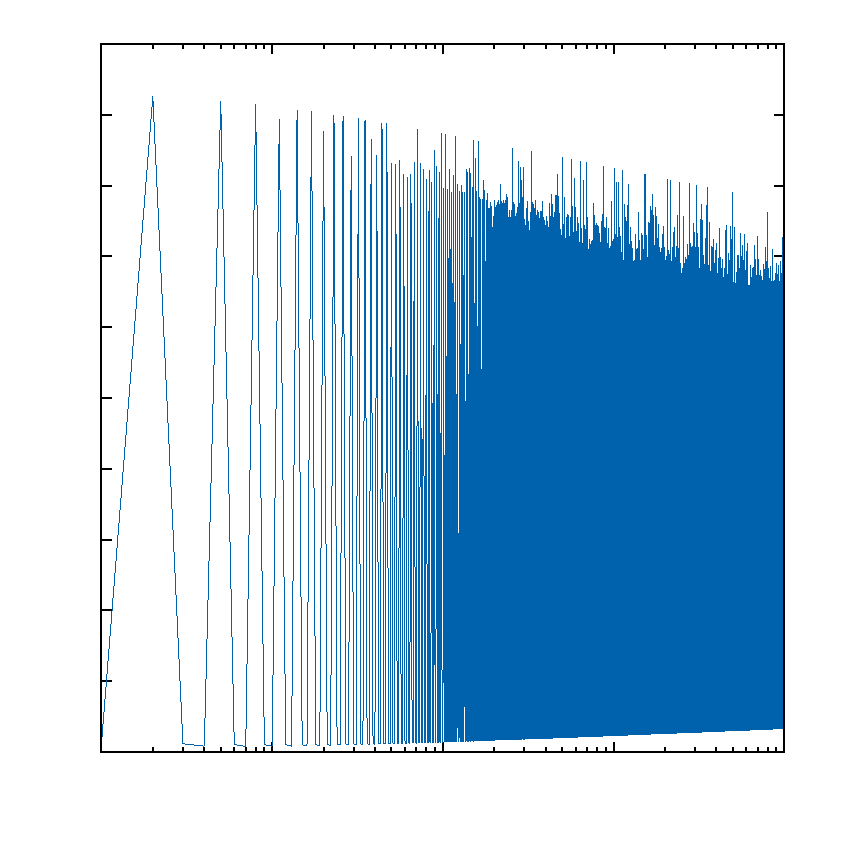
\includegraphics{D:/PhD/Tasks/004/report/secondsincnterror}}%
    \gplfronttext
  \end{picture}%
\endgroup

\caption{Plot of log\textsubscript{10}$E$ versus log\textsubscript{10}$N$ for
numerical differentiation of second derivative using central difference method}
\end{figure}
\newpage
\section*{Numerical solution for 1D heat transfer}
Forward time center in space (FTCS) method was used with the following formula:
\begin{equation}
T_i^{n+1} = T_i^n + \Delta t(\alpha \frac{\partial^2T}{\partial x^2})
\end{equation}
\end{document}